% last updated in April 2002 by Antje Endemann
% Based on CVPR 07 and LNCS, with modifications by DAF, AZ and elle, 2008 and AA, 2010, and CC, 2011; TT, 2014; AAS, 2016

\documentclass[runningheads]{llncs}
\usepackage{graphicx}

\usepackage{amsmath,amssymb} % define this before the line numbering.
\usepackage{mathtools}
\usepackage{xfrac}

\usepackage{algorithm}
\usepackage{algpseudocode}

\usepackage{ruler}
\usepackage{color}
\usepackage[width=122mm,left=12mm,paperwidth=146mm,height=193mm,top=12mm,paperheight=217mm]{geometry}
\begin{document}
% \renewcommand\thelinenumber{\color[rgb]{0.2,0.5,0.8}\normalfont\sffamily\scriptsize\arabic{linenumber}\color[rgb]{0,0,0}}
% \renewcommand\makeLineNumber {\hss\thelinenumber\ \hspace{6mm} \rlap{\hskip\textwidth\ \hspace{6.5mm}\thelinenumber}}
% \linenumbers
\pagestyle{headings}
\mainmatter
\def\ECCV16SubNumber{***}  % Insert your submission number here

\title{Incorporating Multi-Scale Analysis For Depth Estimation} % Replace with your title

\titlerunning{ECCV-16 submission ID \ECCV16SubNumber}

\authorrunning{ECCV-16 submission ID \ECCV16SubNumber}

\author{Anonymous ECCV submission}
\institute{Paper ID \ECCV16SubNumber}


\maketitle

\begin{abstract}
Convolutional neural networks exhibit exceptional performance in predicting depth from stereo images. However, this performance comes with two essential drawbacks (a) they consume extraordinary computational power (clusters of GPUs) even for a single prediction (b) their memory and computational demand is preset from the training phase and cannot be altered at test time according to the capacities/needs of each application.
For confronting these problems, we propose a scalable CNN architecture - MSNet - that adjusts to the specific requirements of each application; it can reduce its computational cost by sacrificing some precision or target for high accuracy if more computational resources are available. This preference for accuracy vs efficiency is determined at test time, without any need for retraining. For achieving this scalability,  we adopted the basic ideas of scale-space theory and adjusted them into the MSNet architecture.
Finally, we compare MSNet to the state-of-the-art methods in the SceneFlow dataset, exhibiting challenging performance using considerably less learnable parameters. 

\keywords{Depth Estimation, Stereo Vision, Deep Learning, Multi-Scale Processing}
\end{abstract}

%%%%%%%%%%%%%%%%%%%%%%%%%%%%%%%%%%%%%%%%%%%%%%%%%%%%%%%%%%%%%%%%%%%%%%%%%%%%%%%%%%%%%%%%%%%%%%%%%%%%%%%%%%%%%%%%%%%%%%%%%%%%%%%%%%%%%%%%%%%%%%%%%%%
\section{Introduction}

Stereo vision forms a particular case of the general 3D reconstruction problem. Stereo cameras share the same orientation while their center is displaced horizontally by a distance $B$. The following relation expresses stereo vision's 3D geometry:

\begin{equation} \label{eq:stereo_geometry}
z = f\frac{B}{d}
\end{equation}

where $z$ is the distance from the camera level (depth), $f$ is the focal length of the camera and $d$ is the disparity. Defining the stereo pair as $X = (X^L, X^R)$, the stereo problem demotes in finding all correspondences $X^L(x,y) \leftrightarrow X^R(x-d, y), \forall (x,y)$.

%%%%%%%%%%%%%%%%%%%%%%%%%%%%%%%%%%%%%%%%%%%%%%%%%%%%%%%%%%%%%%%%%%%%%%%%%%%%%%%%%%%%%%%%%%%%%%%%%%%%%%%%%%%%%%%%%%%%%%%%%%%%%%%%%%%%%%%%%%%%%%%%%%%
\section{Related Work}

Reconstructing the three dimensional geometry from a set of $2D$ images is a core problem of computer vision. Stereo reconstruction is a predominant technique of the aforementioned domain and has been heavily studied over years \cite{Barnard1982ComputationalStereo},\cite{Brown2003}. Scharstein and Szeliski \cite{Scharstein2001AAlgorithms} propose a general taxonomy framework for describing and analysing any stereo vision algorithm in four steps: matching cost computation, cost aggregation, disparity computation/optimisation and disparity refinement.

The matching cost computation realises a dissimilarity measurement between each pixel on reference image and all possible corresponding locations. Quite a lot of metrics of dissimilarity have been proposed, including  absolute difference, squared difference, cross correlation and hamming distance. Dissimilarity metrics can be applied on many different local descriptors, such as LoG, CENSUS \cite{Zabih1996ACorrespondence} and BRIEF \cite{Calonder2010}. Mutual Information \cite{Viola1997} proposes a rather different metric based on the entropy of histograms of correnspondent locations. An extensive evaluation of different matching cost computation strategies has been proposed by \cite{Hirschmuller2007}. Initial matching costs are error prone due to the intense locality of information. Initial estimates need to get optimized by methods taking into account global image information. This can be accomplished through graph cuts \cite{Kolmogorov}, \cite{Boykov2001} and belief propagation \cite{Klaus2006}. Semi-Global-Matching (SGM) \cite{Hirschmuller2008StereoInformation} attempts to minimize a global energy function.

Stereo vision methods are evaluated on datasets containing ground truth depth or disparity for stereo pairs. Middlebury \cite{Scharstein2014} contains indoor scenes. KITTI \cite{Menze2015ISA}, \cite{Menze2018JPRS} is a larger dataset with outdoor scenes and ground truth labels collected from LIDAR on a moving vehicle. Mayer et. al \cite{Mayer2016ALD} created a big synthetic dataset for training big machine learning models.

Deep convolutional networks show great success on stereo vision problems. Intial deep learning proposals focused on matching cost compuation. Zagoruyko et. al \cite{Zagoruyko2015LearningNetworks} proposed a deep convolutional neural network for comparing image patches. \v{Z}bontar and LeCun \cite{Zbontar_2015_CVPR} trained a deep network for predicting the initial matching scores on $9x9$ image patches, followed by traditional aggregation and refinement methods. Luo et. al \cite{Luo2016EfficientMatching} treated matching scores estimation as a multi-label classification problem.

Shaked and Wolf [12] introduce an initial disparity prediction network pooling global information from cost volume

%%%%%%%%%%%%%%%%%%%%%%%%%%%%%%%%%%%%%%%%%%%%%%%%%%%%%%%%%%%%%%%%%%%%%%%%%%%%%%%%%%%%%%%%%%%%%%%%%%%%%%%%%%%%%%%%%%%%%%%%%%%%%%%%%%%%%%%%%%%%%%%%%%%
\section{Multiscale Analysis}

In this section, we discuss the two-fold advantage of incorporating multiscale analysis for depth estimation; (a) it improves the accuracy of patch matching and (b) it offers the tools for designing a scalable model.

\subsection{Multiscale Analysis Improves Patch Matching}

Disparity estimation is based on the hypothesis that the local context of correspondent points is similar. If we define as $P_{n \times n}[x,y]$ the  $n \times n$ square patch centered at $X[x,y]$ and $g(\cdot)$ a metric of patch similarity, then we hope that:

\begin{equation}
\begin{gathered} \label{eq:similarity_hypothesis}
    g(P^L_{n \times n}[x,y], P^R_{n \times n}[x-d^*,y]) > g(P^L_{n \times n}[x,y], P^R_{n \times n}[x-d,y]) \\
    \forall d \in [0,D] : d \neq d^*, \text{where $d* = Y[x,y]$}
\end{gathered}
\end{equation}

For hypothesis \ref{eq:similarity_hypothesis} to hold, we must choose thoughtfully two critical parameters that depend on the specific properties of the points under comparison. 

Firstly, we must select the patch size correctly. For example, regions without texture require a large patch size, so that features from neighboor objects to be included in the compared region. On the other hand, for matching a small foreground object a small patch is appropriate since background objects add noise to the comparison.

The second parameter that we have to adjust is the scale of the comparison. The physical properties of an object (i.e. size), as well as the capturing procedure (i.e. distance from the object, angle), specify the appropriate scale for the patch matching. 

In figure \ref{fig:multiscale_importance_2D}, we design a simple artificial example to show that the task of patch matching is heavily dependent on choosing the correct scale.

We are dealing with both problems using multi-scale patch matching. We keep the patch size constant in terms of number of pixels, but we apply the patch matching procedure sequentially in downscaled and downsampled versions of the initial images. Thus, we apply the matching procedure in many scales and many different neighboor information. Afterwards we aggregate the comparison information from multiple scales.

\begin{figure}[t]
    \begin{center}
        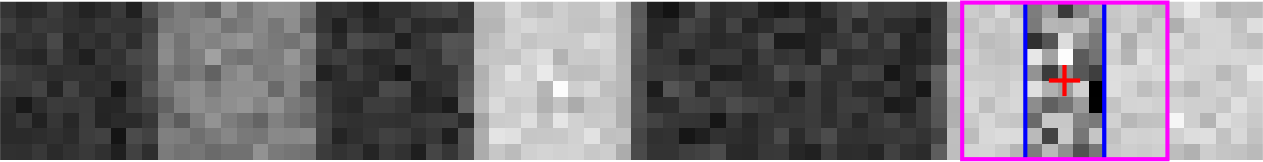
\includegraphics[width=0.49\textwidth]{figures/high_resolution_success_imL_fine.png}
        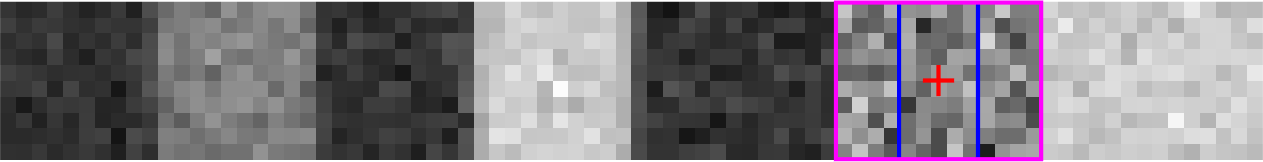
\includegraphics[width=0.49\textwidth]{figures/low_resolution_success_imL_fine.png}\\
        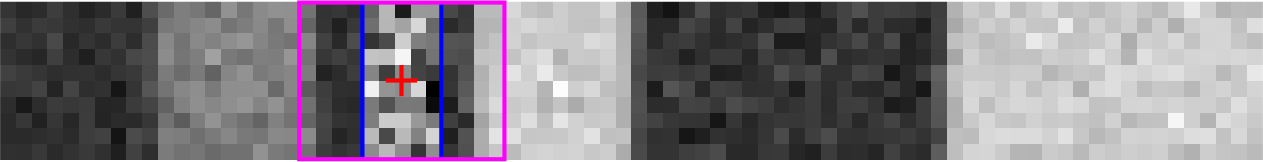
\includegraphics[width=0.49\textwidth]{figures/high_resolution_success_imR_fine.png}
        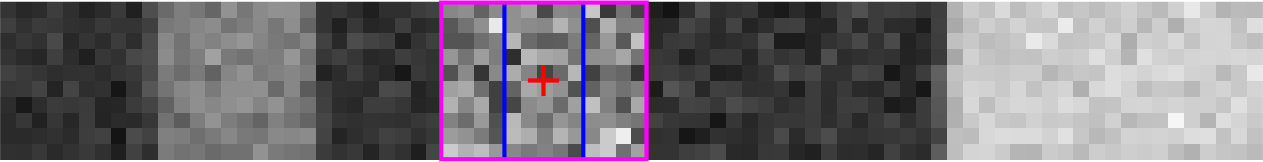
\includegraphics[width=0.49\textwidth]{figures/low_resolution_success_imR_fine.png}\\
        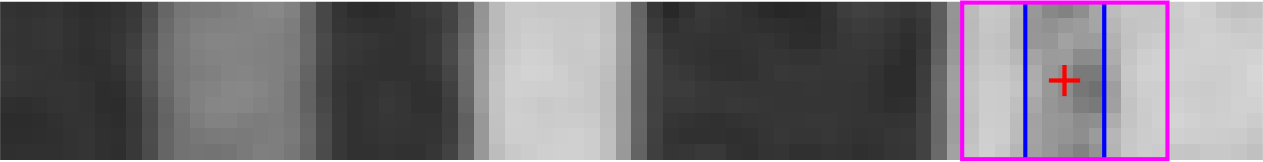
\includegraphics[width=0.49\textwidth]{figures/high_resolution_success_imL_coarse.png}
        
\includegraphics[width=0.49\textwidth]{figures/low_resolution_success_imL_coarse.png}\\
        
\includegraphics[width=0.49\textwidth]{figures/high_resolution_success_imR_coarse.png}
        
\includegraphics[width=0.49\textwidth]{figures/low_resolution_success_imR_coarse.png}\\
        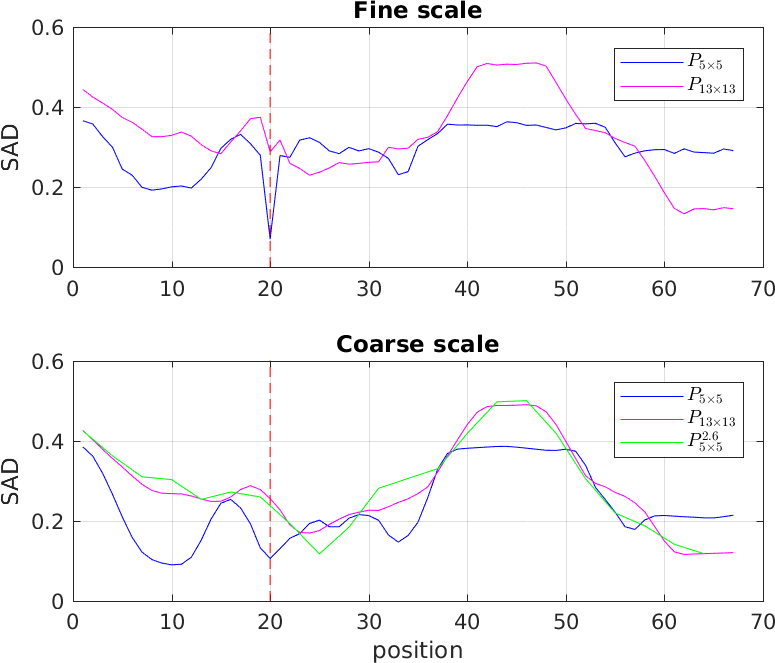
\includegraphics[width=0.49\textwidth]{paper/latex/figures/high_resolution_success_graph.png}
        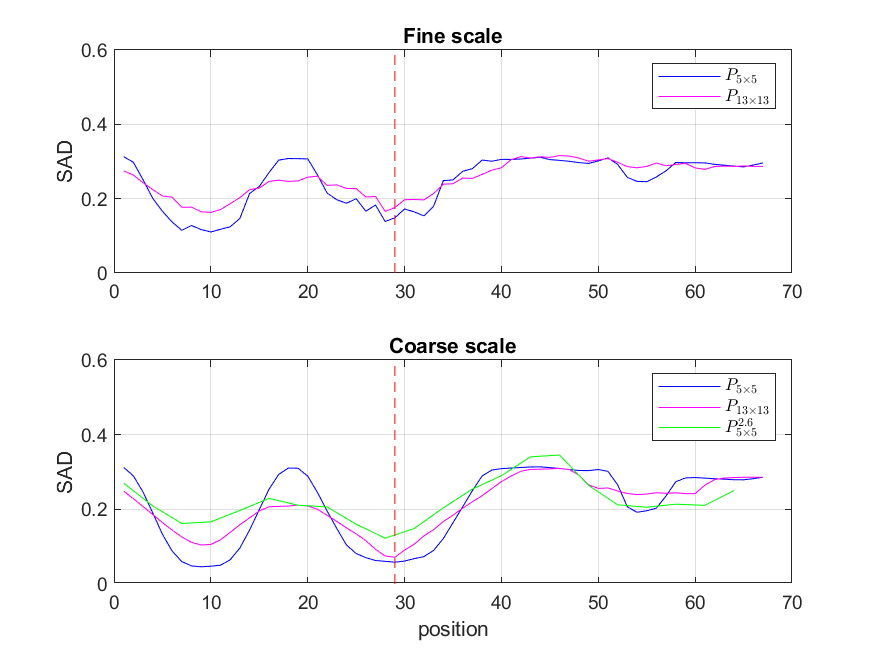
\includegraphics[width=0.49\textwidth]{paper/latex/figures/low_resolution_success_graph.png}\\
        
    \end{center}
    
    \caption{In this figure, we draw a simple artificial example to demonstrate the importance of multiscale patch comparison. In the left column, the fine scale image combined with a small patch size $P_{5 \times 5}$ leads to an accurate disparity curve, whereas in the right example, this happens through the coarse scale and the bigger patch $P_{13 \times 13}$. In the right example, we can observe, that we can approach the same disparity curve by applying a small patch size ($5 \times 5$) after downsampling the coarse scale image at a rate $\sfrac{13}{5}$. This example verifies that instead of keep changing the patch size, we can keep it fixed and apply it to a scale-space pyramid of the stereo pair.}
    \label{fig:multiscale_importance_2D}
\end{figure}

\subsection{Multiscale Analysis Enables A Scalable CNN Architecture}

Multiscale analysis provides the tools for designing an agile CNN architecture that can be readjusted between efficiency and accuracy at test time (i.e. without repeating the training procedure). The learnable parts of the CNN can be repeated between the processing scales that are defined at test time. Thus, if we seek for efficiency and a rough estimation of the depth, we can tune the network to operate at coarse scales. Conversely, if accuracy is the priority, we will set the network to add fine scales, so that the depth estimation will include higher-resolution detail.

\subsection{MSNet architecture}

MSNet comprises of smaller building blocks (modules), which we analyse in this section. We name as $f_*$ the modules that contain learnable parameters and as $g_*$ the ones without learnable parameters. Table \ref{tab:entity_description} defines the tensors that are inputs/outputs of the modules. Figure \ref{fig:cnn_architecture} provides a visual description of all the modules that are part of the architecture.

\subsubsection{Downscaling Module - $g_1$}

The module $g_1^t : \mathbb{R}^{H \times W} \rightarrow \mathbb{R}^{\sfrac{H}{t} \times \sfrac{W}{t}}$ creates a downscaled stereo pair, where $t$ is the downscaling factor. 

\begin{equation} \label{eq:g1}
    (X^{L,t}, X^{R,t}) = (g_1^t(X^L), g_1^t(X^R))
\end{equation}{}

Specifically, $g_1^t$ convolves the stereo image $X^{\{L|R\}}$ with a Gaussian kernel 

\begin{gather} \label{eq:g1_kernel}
    k(x, y, \sigma) = \frac{1}{2\pi\sigma^2} \cdot e^{\sfrac{-(x^2 + y^2)}{2\sigma^2}} \\
    x,y \in \{-\lceil 4*\sigma + 0.5 \rceil, ..., \lceil 4*\sigma + 0.5 \rceil\}, \sigma = \sfrac{t}{3}
\end{gather}

and afterwards applies bilinear downsampling. In MSNet, $t$ is set to the following list of values $ T = \{ 2^2, 2^3, 2^4, 2^5 \}$ but in general they can be defined to be any positive number. 


\subsubsection{Feature Extraction Module - $f_1$}

The module $f_1: \mathbb{R}^{H \times W \times 3} \rightarrow \mathbb{R}^{H \times W \times K}$ is the CNN responsible for extracting local features for each point of the stereo images. This process is done separately for each stereo image and scale.

\begin{equation} \label{eq:f_1}
    (X^{L,t}_{desc}, X^{R,t}_{desc}) = (f_1(X^{L,t}), f_1(X^{R, t}))
\end{equation} 

\subsubsection{Module For Creating The Comparison Volume - $g_2$}

The module $g_2: (\mathbb{R}^{H \times W \times K}, \mathbb{R}^{H \times W \times K}, \mathbb{R}^{H \times W \times 3}) \rightarrow \mathbb{R}^{D \times H \times W \times (K+3)}$ is used for zipping comparison information into a 3D tensor, the comparison volume $C^t$. Normally, the comparison volume is formed by simply concatenating the descriptors in each disparity position. This approach introduces significant redundancy; the comparison volume with dimensionality $D \times H \times W \times 2K$ is builded by repeating only $H \times W \times 2K$ unique values. For reducing such redundancy, we design a new comparison metric between two scalar features:

\begin{equation} \label{eq:m}
    m: \mathbb{R}^2 \rightarrow \mathbb{R}: m(a_1, a_2) = \frac{|a_1| + |a_2|}{2} \cdot e^{-|a_1 - a_2|}    
\end{equation}


The second term $e^{-|a_1 - a_2|} \in (0,1]$ measures the existence of a feature in both patches and the first term $\frac{|a_1| + |a_2|}{2}$ how intense is the feature in each patch (i.e. $0$ signifies the feature does not exist). Finally, we concatenate the raw left image $X^L$ along the $d$ axis of the comparison volume, in order to save the local context.

\begin{gather} \label{eq:comparison_volume}
    C^t[d, x, y, i] = m( X^{L, t}_{desc}[x,y,i], X^{R, t}_{desc}[x-d,y, i]) \\
    C^t \leftarrow X^{L, t} \oplus C^t
\end{gather}

\subsubsection{Module For Processing The Comparison volume - $f_2$}


\subsubsection{Multiscale Fusion Module}

This module is responsible for exploiting information from different scales and merge it in a single comparison volume. The procedure takes place recursively in pairs of two, from coarse to fine scales; a coarse (low resolution) scale is getting merged with a fine (higher resolution) until the highest resolution is reached. The goal of the learnable module $f_3$ is to understand which scale includes the most reliable information and carry it forward to the next level. After multiscale fusion has been completed, the output tensor $Q^{\{t_0, t_1, \cdot \cdot \cdot, t_n\}}$, which has the same dimensions as $Q^{t_0}$, contains accumulated information from all single-scale tensors. 

Apart from the learnable $f_3$ module, a trilinear upsampling layer 

$$g_3^t: \mathbb{R}^{D \times H \times W \times K} \rightarrow \mathbb{R}^{tD \times tH \times tW \times K}$$ where $t$ represents the upsampling factor, is being used. 

Equation \ref{eq:two_scale_fusion} explains how the scale $i$ is being adopted in the multiscale fusion procedure and the end-to-end explanation of the algorithm is given in \ref{alg:multi_scale_fusion}:

\begin{equation} \label{eq:two_scale_fusion}
Q^{ \{ t_i, \cdot \cdot \cdot, t_{n} \} } = f_3(Q^{t_i} \oplus g_3^{\sfrac{t_i}{t_{i-1}} }(Q^{ \{ t_{i-1}, \cdot \cdot \cdot, t_n \} }))
\end{equation}


\begin{algorithm}
\caption{Multi-scale fusion}\label{alg:multi_scale_fusion}
\begin{algorithmic}[1]
\Procedure{multi scale fusion}{$ Q^{t_0}, Q^{t_1}, \cdot \cdot \cdot, Q^{t_n} $} $\rightarrow Q^{\{t_0, t_1, \cdot \cdot \cdot, t_n\}}$ 
\State $Q \gets Q^{t_n}$ \Comment{Initialize}
\For { \texttt{i=n-1;-1;0} }
\State $Q \gets g_3^{\sfrac{ t_{i+1} }{ t_i } }(Q)$ \Comment{3D Upsampling}
\State $Q \gets Q^{t_i} \oplus Q$ \Comment{Concatenation}
\State $Q \gets f_3(Q)$ \Comment{Merge information}
\EndFor
\State \Return $Q^{\{t_0, t_1, \cdot \cdot \cdot, t_n\}} \gets Q$ \Comment{Result}
\EndProcedure
\end{algorithmic}
\end{algorithm}


\subsubsection{Depth Prediction Module- $f_4$}

The module $f_4: \mathbb{R}^{D \times H \times W \times K} \rightarrow \mathbb{R}^{D \times H \times W}$ is responsible for predicting a vector of probabilities for each possible disparity:

\begin{equation}
S^{\{ t_0, \cdot \cdot \cdot, t_n \}} = f_4(Q^{\{t_0, t_1, \cdot \cdot \cdot, t_n\}})    
\end{equation}{}

A softmax operator applied alond the disparity dimension produces the final prediction:

\begin{equation}
Y^{\{ t_0, \cdot \cdot \cdot, t_n \}} = softargmax_d(S^{\{ t_0, \cdot \cdot \cdot, t_n \}})    
\end{equation}{}


\subsubsection{Putting all pieces together}

MSNet comprises of 4 CNN modules - $f_1, f_2, f_3, f_4$, which are repeated for extracting information at multiple scales and then combine it for producing a single prediction image. At training time, we fix the list of scales to $T = \{ 2^0, 2^1, 2^2, 2^3 \}$. At test time, this list can be changed depending on the specific application needs. For example, if the application lacks computational resources and targets to a quick and rough depth estimation, the scale-list can be set to $T = \{ 16, 32, 64\}$. Vice-versa, if the application needs accuracy and high-resolution detail the list can be set to $T = \{1, 2, 4, 8 \}$.

\begin{equation}
\begin{gathered} \label{eq:full_MSNet_model}
    (X^{L,t_i}, X^{R,t_i}) = (g_1^{t_i}(X^L), g_1^{t_i}(X^R)) \\
    (X^{L,t_i}_{desc}, X^{R,t_i}_{desc}) = (f_1(X^{L,t_i}), f_1(X^{R, t_i})) \\
    C^{t_i} = g_2(X^{L,t_i}_{desc}, X^{R,t_i}_{desc}, X^{L,t_i}) \\
    Q^{t_i} = f_2(C^{t_i}) \\
    Q^{\{t_0, t_1, \cdot \cdot \cdot, t_n\}} = MultiScaleFusion(Q^{t_0}, Q^{t_1}, \cdot \cdot \cdot, Q^{t_n}) \\
    S^{\{ t_0, \cdot \cdot \cdot, t_n \}} = f_4(Q^{\{t_0, t_1, \cdot \cdot \cdot, t_n\}}) \\
    Y^{\{ t_0, \cdot \cdot \cdot, t_n \}} = g_4(softargmax_d(S^{\{ t_0, \cdot \cdot \cdot, t_n \}})) \\
    
\end{gathered}
\end{equation}


\subsection{Cnn architectures}

In this section we present the CNN architectures used as the learnable parts of our model. 

\begin{figure}[t]
    \centering
    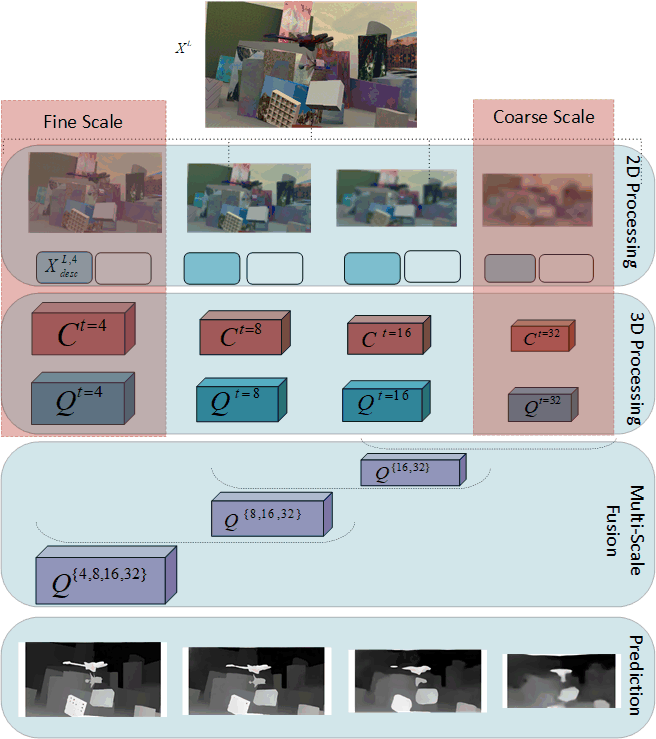
\includegraphics[width = \textwidth]{figures/stereo_architecture.png}
    \caption{Scale fusion network overview. Its main constructive blocks are the horizontal pipelines (green colour) representing end-to-end predictions at specific scale $\sigma$ and the vertical pipelines (grey colour) representing the pair-scales fusion at similarity matrix level. The red-coloured blocks are the learned parts of our architecture, while the yellow coloured ones are hand-crafted layers.}
    \label{fig:cnn_architecture}
\end{figure}

\begin{table}[t]
    \centering
    \begin{tabular}{ l|c|c }
    Description & Symbol & Set \rule{0pt}{2ex}\\
    
    \hline
    \multicolumn{3}{c}{ \textbf{Definitions} } \rule{0pt}{2.4ex}\\
    \hline
    
    Raw image & $X^L, X^R$ & $\mathbb{R}^{H \times W \times 3}$ \rule{0pt}{2.5ex} \\
    
    Ground truth & $Y$ & $\mathbb{R}^{H \times W}$ \rule{0pt}{2.5ex} \\
    
    \hline
    \multicolumn{3}{c}{ \textbf{Single-Scale 2D Processing} } \rule{0pt}{2.4ex}\\
    \hline
    
    Downscaled image & $X^{L,t}, X^{R, t}$ & $\mathbb{R}^{\sfrac{H}{t} \times \sfrac{W}{t} \times 3}$ \rule{0pt}{3ex} \\
    
    Descriptor image at scale $t$ & $X^{L,t}_{desc}, X^{R, t}_{desc}$ & $\mathbb{R}^{\sfrac{H}{t} \times \sfrac{W}{t} \times K}$ \rule{0pt}{3.5ex} \rule[-1.3ex]{0pt}{0pt}\\
    
    \hline
    \multicolumn{3}{c}{ \textbf{Single-Scale 3D Processing} } \rule{0pt}{2.4ex}\\
    \hline
    
    Comparison volume & $C^{t}$ & $ \mathbb{R}^{ \sfrac{D}{t} \times \sfrac{H}{t} \times \sfrac{W}{t} \times K } $ \rule{0pt}{3ex} \\
    
    Processed comparison volume & $Q^{t}$ & $ \mathbb{R}^{ \sfrac{D}{t} \times \sfrac{H}{t} \times \sfrac{W}{t} \times K } $ \rule{0pt}{3ex} \\
    
    Similarity volume & $S^{t}$ & $ \mathbb{R}^{ \sfrac{D}{t} \times \sfrac{H}{t} \times \sfrac{W}{t}} $  \rule{0pt}{3.5ex} \\
    
    Prediction image & $\hat{Y}^{t}$ & $\mathbb{R}^{H \times W}$ \rule{0pt}{3.5ex} \\
    
    \hline
    \multicolumn{3}{c}{ \textbf{Multi-Scale 3D Processing} } \rule{0pt}{2.4ex} \\
    \hline
    
    Comparison volume & $C^{ \{ t_0, ... , t_n \} }$ & $ \mathbb{R}^{ \sfrac{D}{t_0} \times \sfrac{H}{t_0} \times \sfrac{W}{t_0} \times K }  $ \rule{0pt}{3ex} \\
    
    Processed comparison volume & $Q^{ \{ t_0, ... , t_n \} }$ & $ \mathbb{R}^{ \sfrac{D}{t_0} \times \sfrac{H}{t_0} \times \sfrac{W}{t_0} \times K }  $ \rule{0pt}{3ex} \\
    
    Similarity volume & $S^{ \{ t_0, ... , t_n \} }$ & $ \mathbb{R}^{ \sfrac{D}{t_0} \times \sfrac{H}{t_0} \times \sfrac{W}{t_0}} $ \rule{0pt}{3.5ex} \\
    
    Prediction image & $\hat{Y}^{ \{ t_0, ... , t_n \} }$ & $\mathbb{R}^{ H \times W}$ \rule{0pt}{3.5ex} \\
    \hline
    \end{tabular}
    \caption{Description of all tensors involved in MSNet. All tensors follow the dimensions defined by their scale, apart from the final prediction image $\hat{Y}$. In this case, the scale (or list of scales) declares the processing scales used in the prediction. The final prediction shares always the same shape with the raw images.}
    \label{tab:entity_description}
\end{table}

%%%%%%%%%%%%%%%%%%%%%%%%%%%%%%%%%%%%%%%%%%%%%%%%%%%%%%%%%%%%%%%%%%%%%%%%%%%%%%%%%%%%%%%%%%%%%%%%%%%%%%%%%%%%%%%%%%%%%%%%%%%%%%%%%%%%%%%%%%%%%%%%%%%
\section{Experimental Evaluation}

\begin{table}[t]
    \centering
    \begin{tabular}{ c|c|c|c|c }
    Method & Parameters (M) & Runtime & MAE & PCG \\
    
    \hline
    \multicolumn{5}{c}{ \textbf{Our benchmark - IMS architectures} } \\
    \hline
    MSNet & 0.743 & 0.32 & 1.017 & 3.98 \\
    \hline
    OneRes (S) & 0.463 & 0.11 & 1.508 & 6.11 \\
    MRes2d (S) & 0.659 & 0.10 & 1.671 & 6.98 \\
    MRes3d (S) & 0.514 & 0.15 & 1.504 & 5.86 \\
    MRes2d3d (S) & 0.677 & 0.3 & 1.897 & 8.078 \\
    \hline
    OneRes (B) & 1.608 & 0.22 & 1.37 & 5.53 \\
    MRes2d (B) & 1.458 & 0.17 & 1.32 & 5.43 \\
    MRes3d (B) & 1.682 & 0.21 & 1.322 & 5.11 \\
    MRes2d3d (B) & 1.772 & 0.32 & 1.613 & 6.67 \\
    \hline
    \multicolumn{5}{c}{ \textbf{Our benchmark - Free weights} } \\
    \hline
    Free2d & 0.969 & 0.24 & 1.126 & 4.33 \\
    Free3d & 2.75 & 0.33 & \textbf{0.882} & \textbf{3.48} \\
    Free2d3d & 2.974 & 0.33 & 1.107 & 4.36 \\
    \hline
    \multicolumn{5}{c}{ \textbf{SOTA} } \\
    \hline
    PSMNet\cite{Chang2018PyramidNetwork} & - & - & 1.09 & - \\
    CRL\cite{Pang2018CascadeMatching} & - & - & 1.32 & - \\
    DispNetC\cite{Mayer2016ALD} & - & - & 1.68 & - \\
    GC-Net\cite{Kendall2017End-to-EndRegression} & 3.5 & 0.95 & 2.51 & 9.34 \\
    Edge-Stereo\cite{SongEdgeStereoResidual} & - & - & 1.12 & 4.99 \\
    CSPN\cite{cheng2018learning} & - & - & 0.78 & - \\
    GA-Net\cite{zhang2019ga} & 2.3 & 1.5 & 0.84 & - \\
    AMNet\cite{du2019amnet} & 4.37 & - & 0.74 & - \\
    
    \hline
    \end{tabular}
    \caption{Model comparison on SceneFlow dataset}
    \label{tab:results}
\end{table}

\begin{figure}[t]
    \begin{center}
        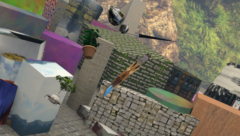
\includegraphics[width=0.24\textwidth,clip]{figures/imL_0.png}
        
\includegraphics[width=0.24\textwidth,clip]{figures/imL_1.png}
        
\includegraphics[width=0.24\textwidth,clip]{figures/imL_2.png}
        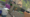
\includegraphics[width=0.24\textwidth,clip]{figures/imL_3.png}
        \\
        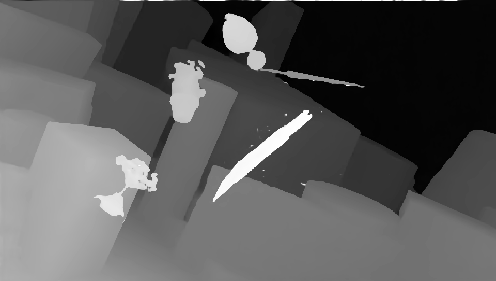
\includegraphics[width=0.24\textwidth,clip]{figures/pred_comb_0.png}
        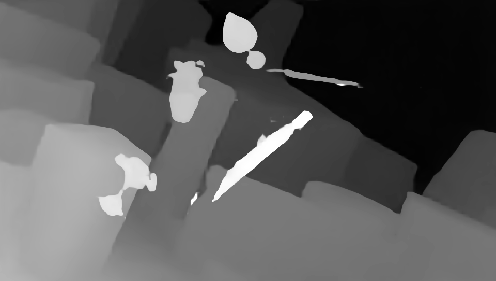
\includegraphics[width=0.24\textwidth,clip]{figures/pred_comb_1.png}
        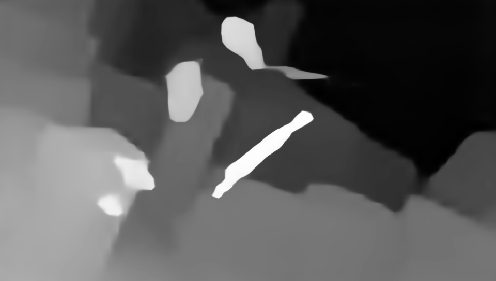
\includegraphics[width=0.24\textwidth,clip]{figures/pred_comb_2.png}
        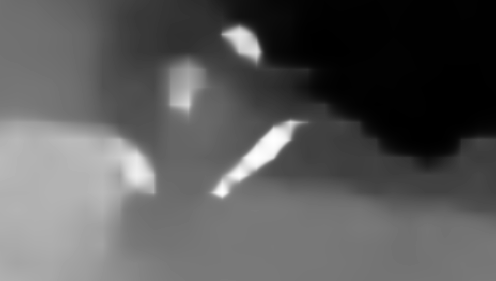
\includegraphics[width=0.24\textwidth,clip]{figures/pred_comb_3.png}
        \\
        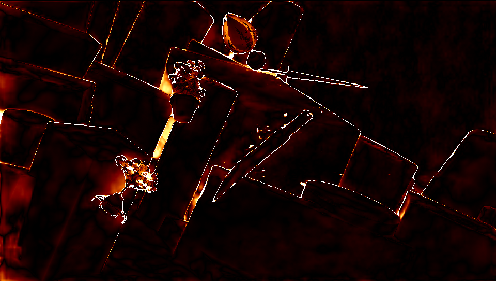
\includegraphics[width=0.24\textwidth,clip]{figures/pred_comb_0_err.png}
        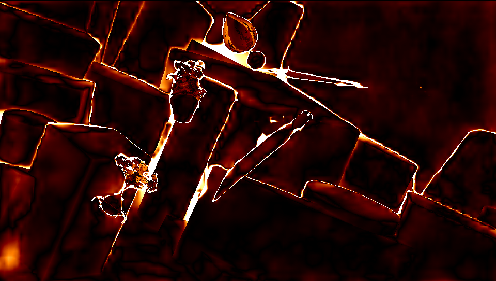
\includegraphics[width=0.24\textwidth,clip]{figures/pred_comb_1_err.png}
        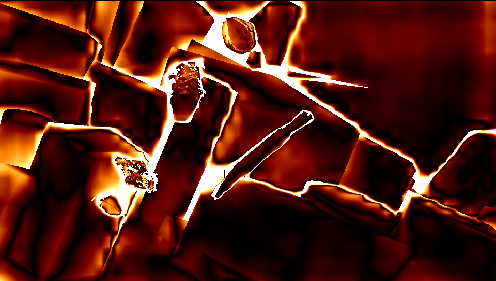
\includegraphics[width=0.24\textwidth,clip]{figures/pred_comb_2_err.png}
        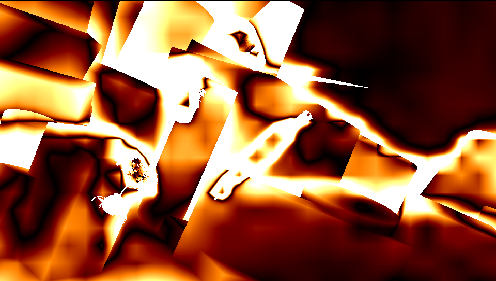
\includegraphics[width=0.24\textwidth,clip]{figures/pred_comb_3_err.png}\\
        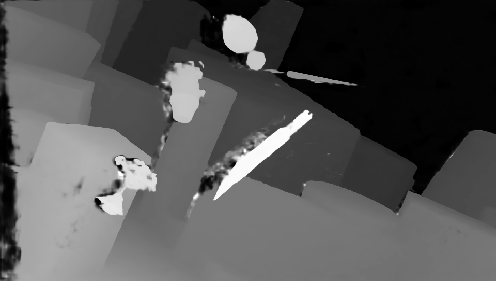
\includegraphics[width=0.24\textwidth,clip]{figures/pred_0.png}
        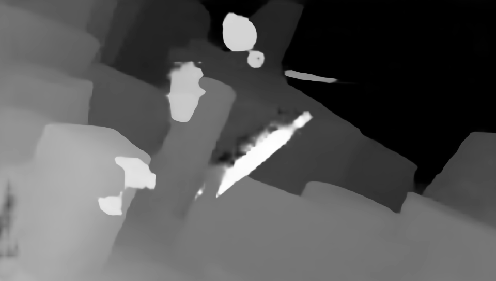
\includegraphics[width=0.24\textwidth,clip]{figures/pred_1.png}
        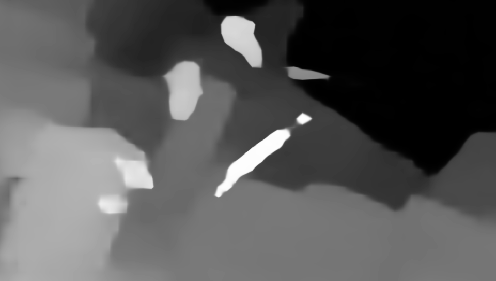
\includegraphics[width=0.24\textwidth,clip]{figures/pred_2.png}
        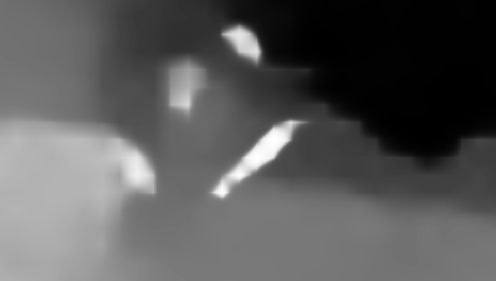
\includegraphics[width=0.24\textwidth,clip]{figures/pred_3.png}
        \\
        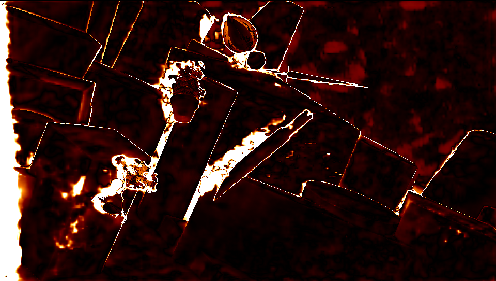
\includegraphics[width=0.24\textwidth,clip]{figures/pred_0_err.png}
        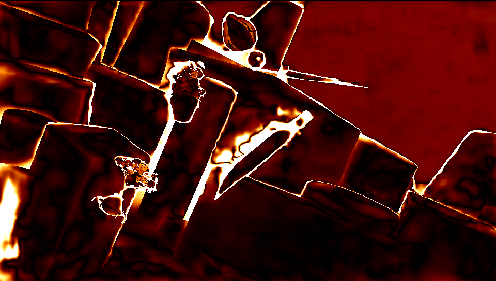
\includegraphics[width=0.24\textwidth,clip]{figures/pred_1_err.png}
        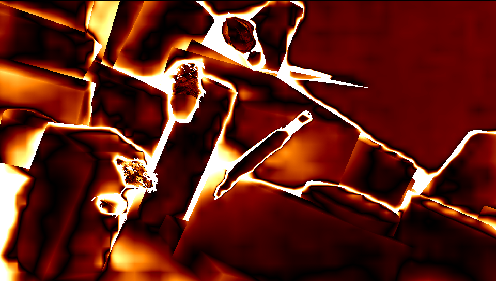
\includegraphics[width=0.24\textwidth,clip]{figures/pred_2_err.png}
        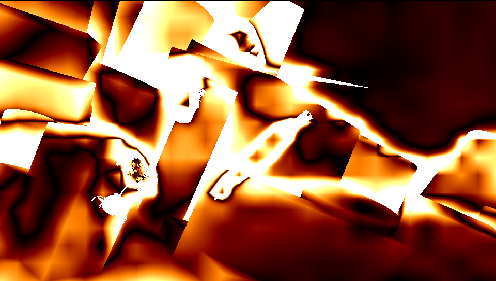
\includegraphics[width=0.24\textwidth,clip]{figures/pred_3_err.png}\\        
    \end{center}
    
    \caption{Text}
    \label{fig:EMAPs}
\end{figure}

In this section we measure the performance of the proposed method on the large synthetic SceneFlow dataset. Table \ref{tab:results} presents the aggregated results of our experiments and figure \ref{fig:EMAPs} the results on a single training example.

\subsection{The Effect Of Using Multi-Scale Processing Explicitly}

In this section, we test whether enforcing multi-scale processing explicitly, as in MSNet, is more beneficial than using multi-scale processing internally as part of the CNN architecture. For this reason, we design 4 new CNN models that follow the MSNet designing principles, but without enforcing multi-scale processing explicitly; Instead, we use the hourglass model (i.e. encoder-decoder architecture) which is the proposed method by the literature, for applying multi-resolution processing internally. The 4 architectures that we desing are the following; OneRes operates only on the initial resolution, MRes2d uses the hourglass model only in the 2D-processing part, MRes3d only in the 3D-processing part and finally MRes2d3d in both the 2D and 3D processing part. For each of the 4 CNNs we create two versions; the small (S) version has the same number of free parameters as MSNet and big (B) has as many parameters as the GPU memory allows. For clarity, we call all these new models with the common name Implicit Multi-Scale (IMS) architectures.

In figure \ref{fig:mae_SFNvsSFN_free_weights} we observe that MSNet outperforms both versions of the IMS architectures, which is a crucial indicator that enforcing multi-scale processing explicitly is beneficial for depth estimation. More specifically, big (B) networks outperform small (S) ones as expecting and using the hourglass architecture in the 3D processing part (MRes3d) gives the best performance.

\begin{figure}[t]
    \centering
    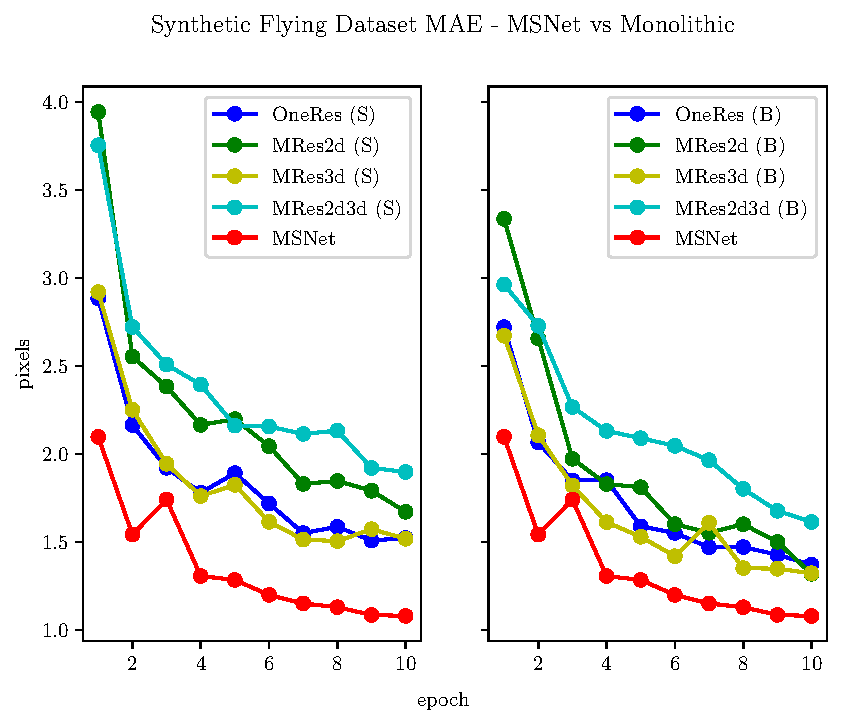
\includegraphics[width=0.7\textwidth]{figures/freiburg_msnet_vs_monolithic_mae.pdf}
    \caption{MSNet comparison with generic architectures}
    \label{fig:mae_SFNvsGenericNets}
\end{figure}

\subsection{What Is the Cost of Sharing Weights}

MSNet is based on the idea of repeating its building blocks $f_1, f_2, f_3, f_4$ along the different scales. Following this principle, it obtains the crucial advantage of being tuned on-demand according to the application needs (accuracy vs computational cost). An important question that arises is how much is the cost in terms of accuracy for gaining such scalability; what would be the corresponding end-point-error (EPE) if we were to apply the backbone architecture of MSNET without weight sharing (i.e. without repeating the same building blocks)? For answering this question, we create a second internal benchmark by implementing three new CNN architectures; MSNet Free2d has free weights only in the 2D-processing part (doesn't repeat $f_1$ blocks), MSNet Free3D has free weights only in the 3D-processing part (doesn't repeat $f_2, f_3, f_4$ building blocks) and, finally, MSNet Free2D3D has free weights end-to-end. The results in the SceneFlow dataset are presented in figure \ref{fig:mae_msnet_vs_free_weights} and in table \ref{tab:results}. We observe that repeating the 3D-processing building blocks ($f_2, f_3, f_4$) through the MultiScaleFusion algorithm leads to a suboptimal solution. Leaving the weights free leads to a better combination of the multi-scale information in the 3D-processing part, leading to an EPE close to the State-Of-The-Art. On the other hand, such approach cancels the scalability advantage of MSNet and is much more memory-intensive.

\begin{figure}[t]
    \centering
    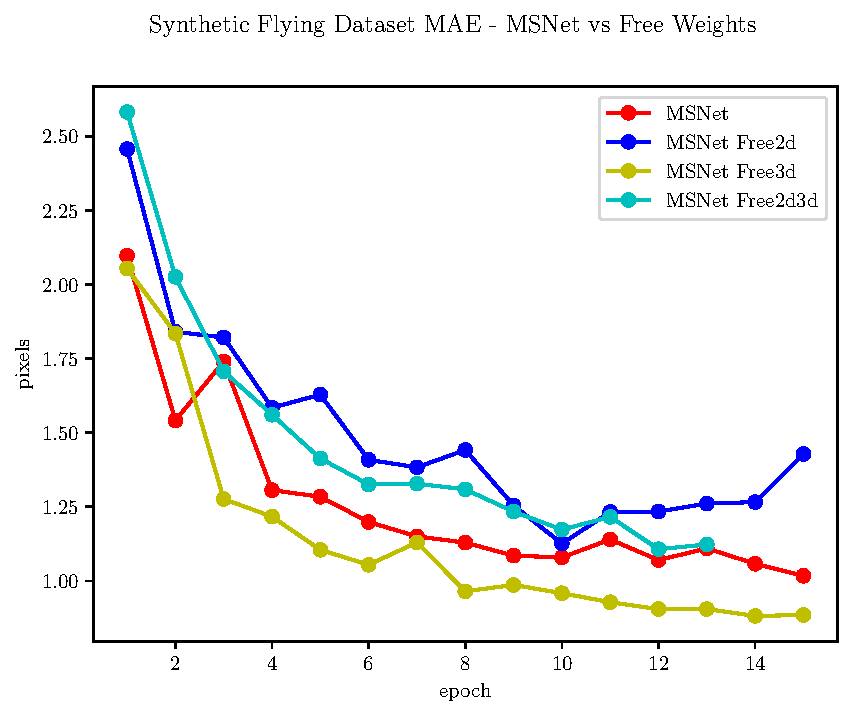
\includegraphics[width=0.5\textwidth]{figures/freiburg_msnet_vs_free_weights_mae.pdf}
    \caption{Text}
    \label{fig:mae_msnet_vs_free_weights}
\end{figure}

\subsection{MSNet vs State-Of-The-Art models}

In table \ref{tab:results}, we can compare the proposed MSNet model with the other SOTA architectures that have been proposed, in the SceneFlow dataset. We observe that MSNet achieves competitive performance (i.e. $1.017$ px of EPE compared to the $0.74$ in \cite{du2019amnet}) even though it uses much less free parameters ($0.7M$ compared to $4.37M$ parameters). This indicates that repeating building blocks along different scales is a beneficial designing principle, that can lead to competitive performance with smaller networks.  

\subsection{MSNet evaluation on different scale combinations}

The fundamental advantage of MSNet compared to other architectures is being able to be tuned between accuracy and efficiency at test time. In figure \ref{fig:msnet_scales_evaluation}, we measure how much the EPE of MSNet varies under using different scales. Firstly, we observe that the EPE and PCG error decreases as we add more scales. Additionaly, the standard deviation $\sigma$ of both EPE and PCG error gets smaller as we add more processing scales, which indicates that by oretaning in more scales we also gain robustness. In general terms adding coarse scales increases the robustness of our predictions, even though the mean EPE may be worse; for example $T=\{ 8 \}$ is better than $ T = \{ 16 \}$ in terms of EPE (i.e. smaller $\mu$ absolute error) but $ T = \{ 16 \}$ has smaller $\sigma$. 

\begin{figure}[t]
    \centering
    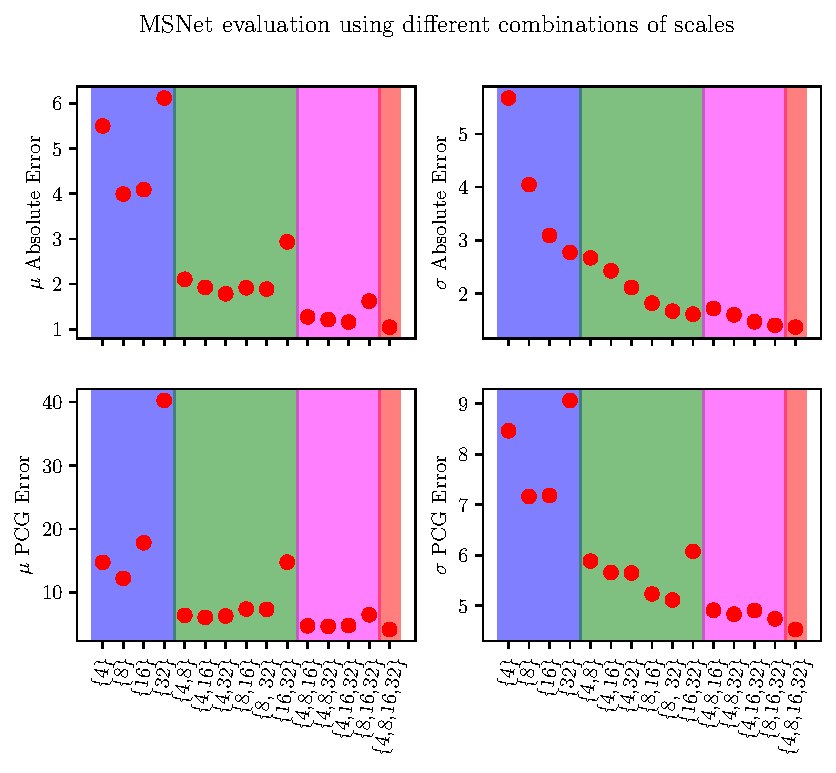
\includegraphics[width=0.8\textwidth]{figures/msnet_scales_evaluation.pdf}
    \caption{MSNet accuracy for different scale combinations. On the x-axis, there are the different scale combinations (i.e. the blue area contains single-scale set-ups, the green area two-scale, the purple area three-scale and the orange area the four-scale combination that was used in the training phase). On the first row we observe the $\mu$ and $\sigma$ of the absolute end-point error and on the second row the $\mu$ and $\sigma$ of the percentage of points with end-point error over 3 pixel.}
    \label{fig:msnet_scales_evaluation}
\end{figure}

\subsection{Multi-Scale fusion analysis} \label{sec:4_1}

In figure \ref{fig:multiscale_importance}, we show how our 3D cnn network has learned incorporating and progressively adopting fine scale predictions. We choose two points with different features; the yellow-box region contains a thin object with texture, which is appropriate for small and high-resolution patch. On the other hand, the orange-box contains a background wall with repetitive pattern, which needs a broader patch containing features from neighbourhood objects. In the orange-box scenario a small, high-resolution patch would lead to a confusion with each neighboor points. For confirming this hypothesis, we initially tune the network for single-scale predictions (i.e. right column in the graph). We can confirm that fine scale works well in the yellow-box and coarse scale in the orange-box region. On the left column, we observe the corresponding results, when the network is set to multi-scale prediction; it achieves accurate predictions in both cases, since it has learned to detect the appropriate scale and rely its prediction on it.

In figure \ref{fig:EMAPs} we present the predictions of the network along with the error images. We observe that initially, at the coarse scale, the network predicts a rough estimation of the depth without many details. As it passes through finer scales, it gradually adopts high-resolution details. This procedure can be seen, as a step-by-step refinement of the initial low-resolution prediction.

\begin{figure}[t]
    \begin{center}
        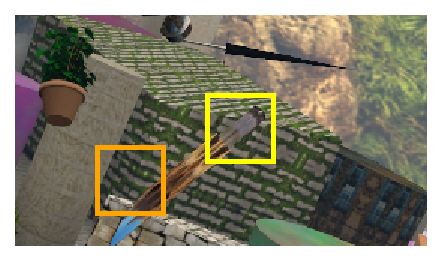
\includegraphics[width=0.49\textwidth]{paper/latex/figures/multiscale_importance_image_patches.pdf}\\
        \includegraphics[width=\textwidth]{paper/latex/figures/multiscale_importance_graph_high_resolution.pdf}\\
        \includegraphics[width=\textwidth]{figures/multiscale_importance_graph_high_resolution.pdf}
    \end{center}
    
    \caption{In this figure, we compare two regions of the same image that require processing on different scale. The centre point of the yellow rectangle is a small object on the foreground with many features (i.e. handle of a knife), whilst the orange one represents a background area inside a repetitive pattern. The first column of graphs represents the Multi-Scale similarity volumes $S^{\{ \sigma_0, ..., \sigma_n \} }$ The graphs prove that, as we expected, disparity estimation is accurate on higher scale for the yellow rectangle and on t As expected,  }
    \label{fig:multiscale_importance}
\end{figure}


\subsection{MSNet evaluation on smaller training set}

In figure \ref{fig:msnet_smaller_tr_set}, we present MSNet performance under training set of different size. As expected, the accuracy increases as the model observes more training data.

\begin{figure}[t]
    \centering
    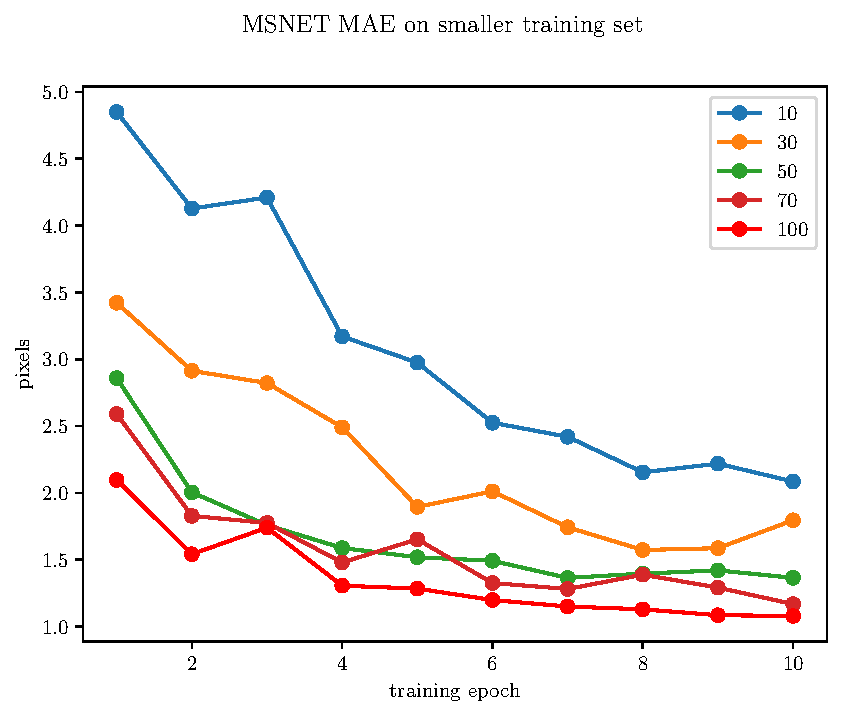
\includegraphics[width=0.5\textwidth]{figures/freiburg_msnet_mae_smaller_training_set.pdf}
    \caption{Caption}
    \label{fig:msnet_smaller_tr_set}
\end{figure}

\bibliographystyle{splncs}
\bibliography{egbib}
\end{document}
